%!TEX root = doc.tex
\section{Future Work}
\label{sec:prototype}

In this section we specify some of the future developments that are planned for \apiname. We also present the tool under development that initially created the need for the development of \apiname.

\subsection{Conversion Tool Prototype}

The goal of the tool we propose is to allow the automatic conversion of Repast simulations into JADE applications. This conversion tool will not only allow the developer to quickly generate a MAS or create a simulation but also enables a proficient programmer in one framework to quickly get started in developing with the other framework. Figure \ref{fig:prototypeFlow} illustrates these two plausible workflows.

\begin{figure}[h]
	\centering
	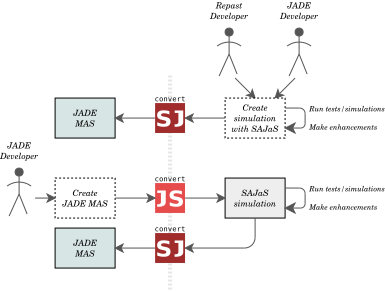
\includegraphics[width=3.0in]{figures/prototypeFlow.pdf}
	\caption{
		Two possible workflows for \apiname{} users
	}
	\label{fig:prototypeFlow}
\end{figure}

The code conversion tool uses the Java Development Tools (JDT) from Eclipse which enables Java programmers to perform introspection and reflection tasks with ease. This approach allows programmers to perform code transformations without having to create parsers for Java code and abstract syntax trees (AST).

The conversion tool will be developed in the form of an Eclipse plug-in, in order to be able to make use of all JDT features.

\subsection{\apiname{} development}

Although \apiname{} is already fit for development of Repast simulations, it's still an ongoing project. One important trait of \apiname{} is that, although tailored for repast, it's very generic. This means that MABS built using other Java simulation tools can integrate our API successfully in the future and, therefore, use Jade-based tools.
